\documentclass[a4paper,11pt]{article}
\pdfoutput=1 % if your are submitting a pdflatex (i.e. if you have
             % images in pdf, png or jpg format)

\usepackage{jcappub} % for details on the use of the package, please
                     % see the JCAP-author-manual

\usepackage[T1]{fontenc} % if needed
% \usepackage{subfig}
\usepackage[utf8]{inputenc}

\usepackage{color}

\newcommand{\ek}[1]{{{\bf \color{red} EK: #1}}}
\newcommand{\re}[1]{{{\bf \color{green} RE: #1}}}

\title{\boldmath The Core-Cusp Problem Revisited: ULDM vs. CDM}


%% %simple case: 2 authors, same institution
%% \author{A. Uthor}
%% \author{and A. Nother Author}
%% \affiliation{Institution,\\Address, Country}

% more complex case: 4 authors, 3 institutions, 2 footnotes

\author[1]{Emily Kendall,}
\author[1]{Richard Easther}


% The "\note" macro will give a warning: "Ignoring empty anchor..."
% you can safely ignore it.

\affiliation[1]{Department of Physics, University of Auckland, Private Bag 92019, Auckland, New Zealand}

% e-mail addresses: one for each author, in the same order as the authors
\emailAdd{eken000@aucklanduni.ac.nz}
\emailAdd{r.easther@auckland.ac.nz}




 
\abstract{The core-cusp problem is often cited as a motivation for the exploration of a wider variety of dark matter models other than standard CDM [cold dark matter]. One such alternative is ULDM [ultra-light dark matter], which  proposes that dark matter consists of ultralight particles exhibiting wavelike properties on kiloparsec scales. ULDM obeys the Schr\"{o}dinger-Poisson equation and has soliton-like solutions consisting of gravitationally bound condensates with no internal kinetic energy; however astrophysically realistic ULDM halos would  consist of a larger NFW-like configurations with a possible solitonic core. The size of this core relative to the outer halo can be approximately calculated based on a well-known core-halo mass relation, however we argue here that this relation should not be taken to be exact. We describe a parameterisation for the radial density profiles of these scenarios which accounts for the environmental variability of the core-halo mass relation of realistic halos, and  compare these to simulated ULDM halos generated numerically by colliding a number of individual solitons; this computationally efficient strategy precludes direct analysis of the evolutionary histories and interactions, but  allows us to create large numbers of prototype halos, with multiple realisations of these scenarios evolving towards broadly similar final states.
Utilising the SPARC database we show that ULDM-only models do not necessarily exacerbate the core-cusp problem relative to standard CDM for the SPARC dwarf galaxies, however we acknowledge that baryonic feedback within galaxies in the SPARC mass range is an important consideration which is not captured here. While we find that a ULDM particle mass of $10^{-23}\operatorname{eV}$ yields a reasonably good fit to a subset of SPARC data, such a small particle mass is in tension with current constraints.}
 


\begin{document}
\maketitle
\flushbottom


\section{Introduction}\label{sec:intro}


 
It is widely agreed that non-baryonic dark matter constitutes the majority of the mass of the observable universe, but its precise nature is one of the most important open questions in fundamental physics. Many dark matter models have been proposed, with CDM [Cold Dark Matter] proposals being the most widely studied. However, while this scenario successfully accounts for the large scale structure of the universe \cite{Springel:2005nw} and the spectrum of anisotropies in the microwave background \cite{deBernardis:2000sbo, Hanany:2000qf, Halverson:2001yy, Netterfield:2001yq, Lee:2001yp, Ade:2015xua,  Hu:2001bc}, the so-called ``small-scale crisis'' \cite{Weinberg:2013aya} remains a challenge. One key issue is the tension between the predicted central density profiles of dark matter halos in simulations containing only gravitationally interacting CDM, and those inferred from observational data. Simulations tend to produce `cuspy' NFW-type central density profiles \cite{Navarro:1995iw}, which go like $1/r$ at small radii, while observational data appears to favour flattened central cores \cite{Moore:1994yx}. This so-called core-cusp problem has been the focus of much recent attention \cite{Dutton:2018nop, Read:2018pft, Genina:2018}. 
 
The seriousness of the core-cusp problem remains the subject of ongoing debate, as it has been shown that the discrepancy may be ameliorated by adding baryonic matter to CDM simulations  \cite{Benitez-Llambay:2018}. Nevertheless, the debate surrounding such `small-scale' problems, along with the discouraging lack of success in direct-detection experiments \cite{Schumann:2019eaa} promotes considerable interest in alternative dark matter models in which central cusps cannot form. One scenario which has gained substantial traction is ultra-light dark matter [ULDM], also known as scalar-field dark matter, $\Psi$ dark matter, axion dark matter, BEC dark matter and fuzzy dark matter. As reviewed by Hui {\em et al.\/} \cite{Hui:2016ltb}, ULDM consists of an axion-like particle whose very small mass  ($\mathcal{O}(\sim 10^{-22}eV)$) corresponds to a kiloparsec-scale de Broglie wavelength. ULDM thus exhibits novel wave-like behaviour on astrophysically interesting scales and can form soliton-like gravitationally confined, Bose-Einstein condensates. ULDM simulations suggest that realistic astrophysical halos have an inner core consisting of a kiloparsec scale Bose-Einstein condensate or soliton, while the outer halo is a virialised system of scalar particles  matching expectations from CDM \cite{Schwabe:2016rze, Veltmaat:2018dfz}. The central regions of the solitonic solutions are relatively flat so it seems that ULDM could  resolve the CDM core-cusp problem without the inclusion of baryonic physics. 

Despite this apparent conceptual success, it has  been argued that in some mass regimes the density profiles predicted by ULDM actually exacerbate the core-cusp problem in comparison to the NFW profiles characteristic of WIMP CDM \cite{Robles:2018fur}. Indeed, as the inner regions of ULDM halos are described by solitonic density profiles, they are subject to the mass scaling laws of the ground-state soliton solutions. This implies that as the mass contained within the central core increases, its radius decreases. For this reason, it is natural to expect that in the most massive cores, a large amount of mass is contained within a small radius. Hence, it is plausible that at small radii the internal mass of a heavy ULDM halo might exceed that of an `equivalent' NFW halo. The authors of \cite{Robles:2018fur} concluded that in comparison to observational data, the NFW profiles of CDM outperform ULDM profiles for dwarf galaxies with masses ($> M_h \sim 10^{11} M_{\odot}$). 

The purpose of this paper is to examine the impact of statistical variation in the core-halo mass scaling relation on the core-cusp discrepancy in ULDM halos. To do this, we utilise the method for constructing a semi-analytic ULDM density profile as developed in \cite{Robles:2018fur}. This method combines a solitonic ULDM core with an NFW-like outer halo to form a `generic' ULDM profile. We test the validity of such synthetic profiles by comparison to numerical density profiles obtained through the PyUltraLight simulation tool \cite{Edwards:2018ccc}.

Accounting for the apparent scatter around the theoretical prediction of the core-halo mass ratio as implied in \cite{Schive:2014hza} and as can be intuitively expected, we find that the core-cusp problem is not necessarily exacerbated for ULDM relative to CDM at scales relevant to dwarf galaxies. This statement, however, relates to dark-matter only simulations. It is known that baryonic feedback in dwarf galaxies can have significant consequences \cite{2018MNRAS.473.5698D, Benitez-Llambay:2018}, and for this reason it is not sensible to disfavour one or the other model based the core-cusp discrepancy of dark-matter alone.

Using dark-matter only models, we find that neither ULDM halos (for ULDM particle mass $0.8-2.5\times 10^{-22} \operatorname{eV}$)
nor NFW halos provide a particularly convincing fit to astrophysical data in the SPARC database \cite{Lelli:2016zqa}. However, we note that the SPARC database is not exhaustive, with measurements for some dwarf galaxies being limited to only a few data points, and many of the profiles having significant uncertainties. The profiles of different objects in the database also vary widely in character, so it would be difficult for any theoretical model to provide a universally good fit. 
These considerations, along with those discussed above, make drawing strong conclusions difficult. Furthermore, looking at numerical simulations we see that while the spherically-averaged density profiles of simulated ULDM halos follow a predictable format, the outer regions are highly turbulent, so that any individual point may vary widely from the global average. These uncertainties notwithstanding, we demonstrate that a ULDM particle mass of $10^{-23}\operatorname{eV}$ can yield a range of plausible ULDM halo profiles which give a reasonable fit to a subset of profiles from the SPARC database, with good agreement at small radii. This very small particle mass, however, is in tension with some recent ULDM constraints. Hence, further investigation is needed to determine whether ULDM can provide a suitable framework within which to describe dwarf galaxies. 

The structure of the paper is as follows. In Section \ref{sec:models}, we review the construction of semi-analytic density profiles for both the ULDM and CDM models. In Section \ref{sec:sim_comparison} we  verify the validity of the semi-analytic ULDM profile  through comparison to simulation data. In Section \ref{sec:ULDM_v_CDM} we compare the semi-analytic density profiles for ULDM and CDM halos in the dwarf galaxy mass range $10^{11} - 10^{12}\operatorname{M}_{\odot}$, taking into account statistical variation in both the NFW concentration parameter and the ULDM core-halo mass relation. Finally, in Section \ref{sec:velocity} we compare the radial velocity profiles inferred from these density profiles with astrophysical data from the SPARC database \cite{Lelli:2016zqa}. We conclude in Section \ref{sec:conclusion}.

%\clearpage





\section{Semi-analytic models of dark matter halos}\label{sec:models}


\subsection{The NFW profile of CDM}

We begin by looking at the semi-analytic parametrisations of ULDM and CDM halo models. The  NFW [Navarro-Frenk-White] profile of CDM \cite{Navarro:1995iw, Maccio:2008pcd}  is well known and given by
%
\begin{equation}\label{eq:nfw}
    \rho_{NFW}(r)=\frac{\rho_0}{\frac{r}{R_s}\left(1+\frac{r}{R_s}\right)^2},
\end{equation}
%
where the parameters $\rho_0$ and $R_s$ vary from halo to halo. $\rho_0$ can be interpreted as a characteristic density, while $R_s$, the scale radius, determines the radius at which the scaling behaviour of the profile transitions from the `small r' to the `large r' limit; $1/r$, and $1/r^3$, respectively.

By assumption, the profile is radially symmetric and it is well known that the corresponding volume integral for the mass would diverge as $r\rightarrow \infty$ if the theoretical profile were continued to arbitrary radius. In practice, however, the halo will have a finite size and this is typically set by the virial radius, which is approximately determined via the spherical top-hat collapse model \cite{White:2000jv, Suto:2015jdt, Herrera:2017epn} describing the collapse of a uniform spherical overdensity in a smooth expanding background. Collapse halts when virial equilibrium is reached, and the resulting virial radius is parametrised by $\Delta_c \rho_c(t)$ where $\rho_c(t)$ is the critical density of the universe at time $t$. It is found that the numerical factor $\Delta_c$ is of order $10^2$ and while different conventions exist, we will take the common value of $\Delta_c = 200$ \cite{Richings:2018} in what follows. 

If we take the virial radius to define the  physical extent of the halo, equation \ref{eq:nfw} completely specifies the density profile for given  $\rho_0$ and $R_s$. For any given virial mass, there is a range of corresponding NFW density profiles, with constraints on $\rho_0$ and $R_s$ emerging from the mass-concentration-redshift relation evident in the results of N-body simulations and observations \cite{Ludlow:2013vxa, Ragagnin:2018enf}. 

\subsection{The piecewise ULDM halo profile}

ULDM dynamics is governed by the Schr{\"o}dinger-Poisson system of coupled differential equations which, in a static background, have the dimensionless form  
%
\begin{align}
    i\dot{\psi} &= -\frac{1}{2}\nabla^2\psi+\Phi\psi \\
    \nabla^2\Phi &= 4\pi \vert \psi\vert^2
\end{align}
%
where $\psi$ is the ULDM wavefunction, $\Phi$ is the Newtonian potential, and the density $\rho \propto |\psi|^2$. The solitonic profile must be found numerically, but once a spherically symmetric  solution $\psi$ with $\psi(0)=1$ is found, a family of solutions ($\psi'$) can be constructed as%
\begin{equation}
    \psi'(x) = \gamma\psi(\sqrt{\gamma}x),
\end{equation}
where $\gamma$ is a scaling parameter. Under this scaling, the dimensionless mass of the soliton is proportional to $\sqrt{\gamma}$, while the dimensionless radius is proportional to $1/\sqrt{\gamma}$. The dimensionless density $\vert\psi\vert^2$ and dimensionless radius $x$ can be transformed into dimensionful quantities by
\begin{align}
    \rho &= \mathcal{M}\mathcal{L}^{-3}\vert\psi\vert^2, \label{eq:density_conv} \\
    r &= \mathcal{L}x, \label{eq:mass_conv}
\end{align}
where
\begin{equation}\label{eq:length}
    \mathcal{L}=\left(\frac{8\pi\hbar^2}{3 m^2H_0^2\Omega_{m_0}}\right)^{\frac{1}{4}}\approx121\left(\frac{10^{-23}\operatorname{eV}}{m}\right)^{\frac{1}{2}}\operatorname{kpc},
\end{equation}
%
and 
%
\begin{equation}\label{eq:mass}
    \mathcal{M}=\frac{1}{G}\left(\frac{8\pi}{3 H_0^2\Omega_{m_0}}\right)^{-\frac{1}{4}}\left(\frac{\hbar}{m}\right)^{\frac{3}{2}}\approx 7\times 10^7\left(\frac{10^{-23}\operatorname{eV}}{m}\right)^{\frac{3}{2}}\operatorname{M}_{\odot}.
\end{equation}

\

 
Ref.~\cite{Robles:2018fur} gives the following piecewise parameterization of the generic ULDM profile 
%
\begin{equation}\label{eq:piecewise}
     \rho(r)=
    \begin{cases}
      \rho_{sol}(r), & 0\leq r \leq r_{\alpha} \\
      \rho_{NFW}(r), & r_{\alpha}\leq r \leq r_{vir},
    \end{cases}
\end{equation}
%
where $\rho_{sol}(r)$ is the appropriately scaled density profile of the ground state soliton solution.  
To construct the ULDM halo profile in accordance with \ref{eq:piecewise}, we must determine the predicted central density, $\rho_c$, of a ULDM halo for a given virial mass, $M_{vir}$.  It has previously been found that there exists a scaling relationship between the mass of the core (and therefore the central density) of a ULDM halo and the overall virial mass of the halo \cite{Schive:2014hza}. There it is argued that the form of a relaxed halo should be determined solely by globally conserved quantities, namely the total energy and mass. This is then converted into an expression relating the core size to the velocity dispersion, and finally to the halo virial mass\footnote{The authors of \cite{Schive:2014hza} suggest the following general expression:
\begin{equation}
    M_c = \alpha \left(\vert E\vert/M\right)^{1/2},
\end{equation}
where the core mass $M_c$ is determined by the total energy, $E$, and the total mass of the halo, $M$ where $\alpha$ is a constant of order unity. They then explain that the right hand side of the equation represents the halo velocity dispersion, while the left hand side  represents the inverse core size due to soliton scaling laws. By invoking the virial condition of the spherical collapse model, the authors then  construct the redshift dependent relationship between the solitonic core mass and the halo virial mass for a ULDM halo.}. The core-halo mass relation can also be understood simply as the condition that the virial velocity of the core is equal to the virial velocity of the halo. The theoretical relation of \cite{Schive:2014hza} at $z = 0$ is  
%
\begin{equation}\label{eq:central_dens}
    \rho_c = 2.94*10^6 \operatorname{M}_{\odot}\operatorname{kpc}^{-3}\left(\frac{M_{vir}}{10^9 M_{\odot}}\right)^{4/3}m_{22}^{2}
\end{equation}
and 
\begin{equation}
    r_c = 1.6 \operatorname{kpc}\left(\frac{M_{vir}}{10^9 M_{\odot}}\right)^{-1/3}\frac{1}{m_{22}},
\end{equation}
where $r_c$ is the radius at which the density drops to half its central value, and $m_{22}$ is defined as $m_{22} \equiv m / 10^{-22} \operatorname{eV}$. Here $m$ is the ULDM particle mass. 


While this gives us a baseline prediction for the central density of a ULDM halo with a specific virial mass, we expect that there will be a range of acceptable central densities, in analogy with the scatter in the concentration parameter of NFW profiles \cite{Maccio:2008pcd}. Indeed, numerical tests of the predicted scaling relation in \cite{Schive:2014hza} indicate a scatter of up to $\pm 50\%$ from the  predicted value of the core mass, $M_c$, the mass contained within  within $r_c$. Furthermore, it is shown in \cite{Veltmaat:2018dfz} that the core density, when analysed with fine temporal resolution, oscillates in amplitude over more than a factor of two. This is unsurprising given that the central cores are not technically stable soliton solutions, existing not in a vacuum but in an ensemble of turbulent waves. Thus, the core-halo mass relation expressed in \ref{eq:central_dens} should not be taken as a strict constraint, but rather a global statistical trend.

The small sample size and limited halo mass range ($ M_{vir} \approx 10^8-10^{11} \operatorname{M}_{\odot}$)  of the data in Ref.~\cite{Schive:2014hza} means it is probably not meaningful to use it to specify a detailed statistical distribution of halos. Indeed, one must be cautious when extrapolating the core-halo mass relation to realistic halos in regions of parameter space which have yet to be explored experimentally. It is difficult to predict, for example, the effect that star formation and feedback will have on the formation of solitonic cores in halos of different masses. Hence, we will here assume a scatter of $\pm 50\%$, noting that future simulations will hopefully lead to improved predictions for this distribution. 

In addition to the variation in peak core density, we expect to see variation in the radius at which the solitonic profile of the ULDM halo transitions into an NFW profile. This is acknowledged in \cite{Robles:2018fur}, and is captured by the parameter $\alpha$, such that the transition radius, $r_{\alpha}$, is given by $r_{\alpha} = \alpha r_c$, where $3 \leq \alpha \leq 4$. We note that the core-halo scaling relation will place astrophysical constraints on the shape of the NFW piece of the ULDM profile, such that we expect that after the soltion-NFW transition, the density will scale approximately as $1/r^3$. In general the solitonic region of the halo should replace the section of the NFW piece which would scale as $1/r$.  


With the allowances for statistical variation in both the central soliton density and the transition radius taken into account, we can now create a range of plausible ULDM halo profiles for a given halo virial mass. To do this, we use the virial mass to predict $\rho_c$. Combined with an assumption for $\alpha$, the solitonic piece of the ULDM profile is then completely specified, and its mass can be calculated. From here, we can calculate the mass in the the NFW tail of the ULDM profile, and by matching the densities of the NFW tail and the inner soliton at the transition radius, the values of the $R_s$ and $rho_0$ parameters of the ULDM profile NFW tail are fully constrained.  



\section{ULDM profiles from simulations}\label{sec:sim_comparison}


\begin{figure}
\begin{tabular}{cc}
{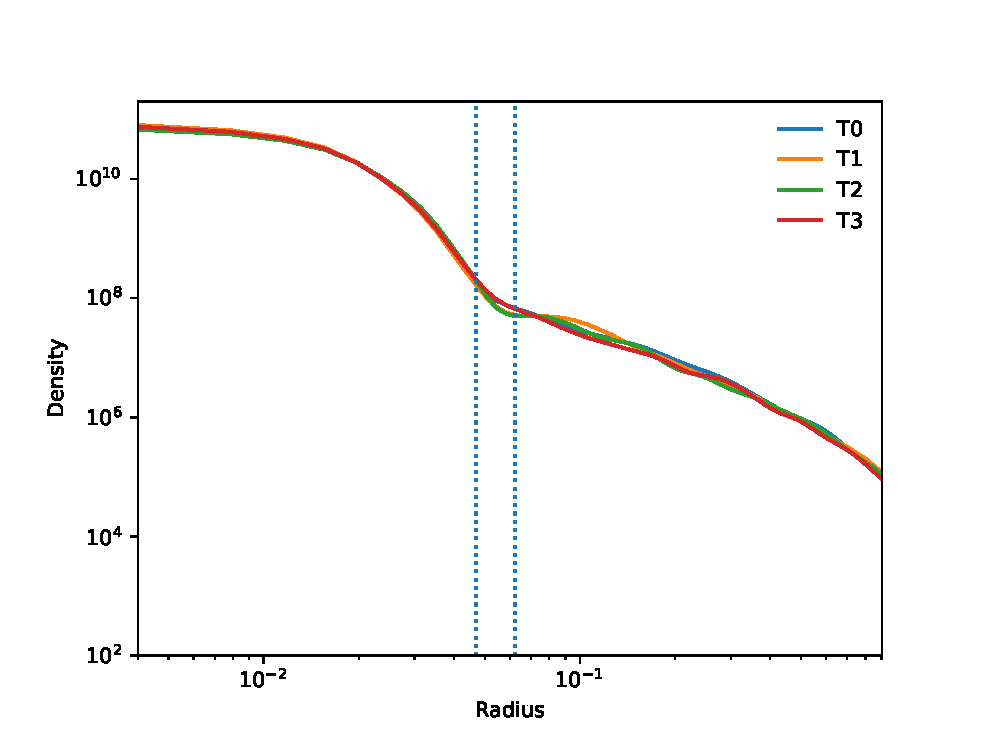
\includegraphics[scale = 0.55, trim={1.5cm 0 0 1cm}]{pics/combined3.eps}} &
{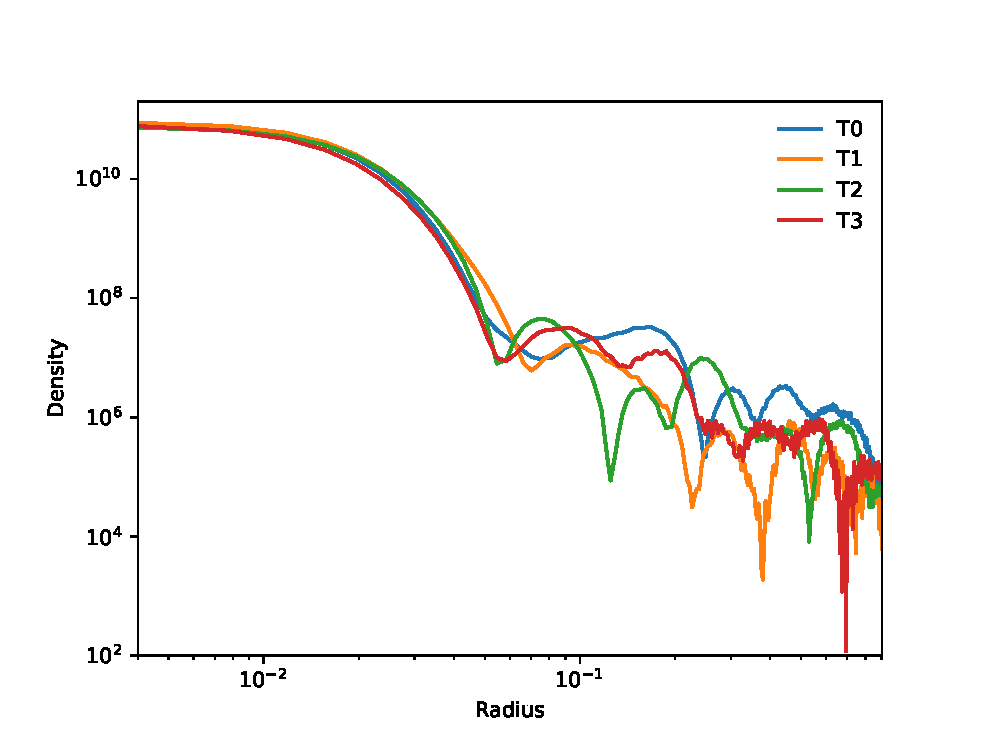
\includegraphics[scale = 0.55, trim={2cm 0 0 1cm}]{pics/singles.eps}}
\end{tabular}
\caption{Left: Spherically averaged density profile of merger product of 8 $\sim 5,000$ code unit solitons. Vertical dotted lines represent 3 and 4 times the core radius (radius at half-maximum density). T1 to T4 represent snapshots at $0.85 \times$ total duration to $1.0 \times$ total duration. 
Right: Density profile along single arbitrary direction. All quantities are represented in dimensionless code units}\label{fig:pul}
\end{figure}

\begin{figure}
\centering
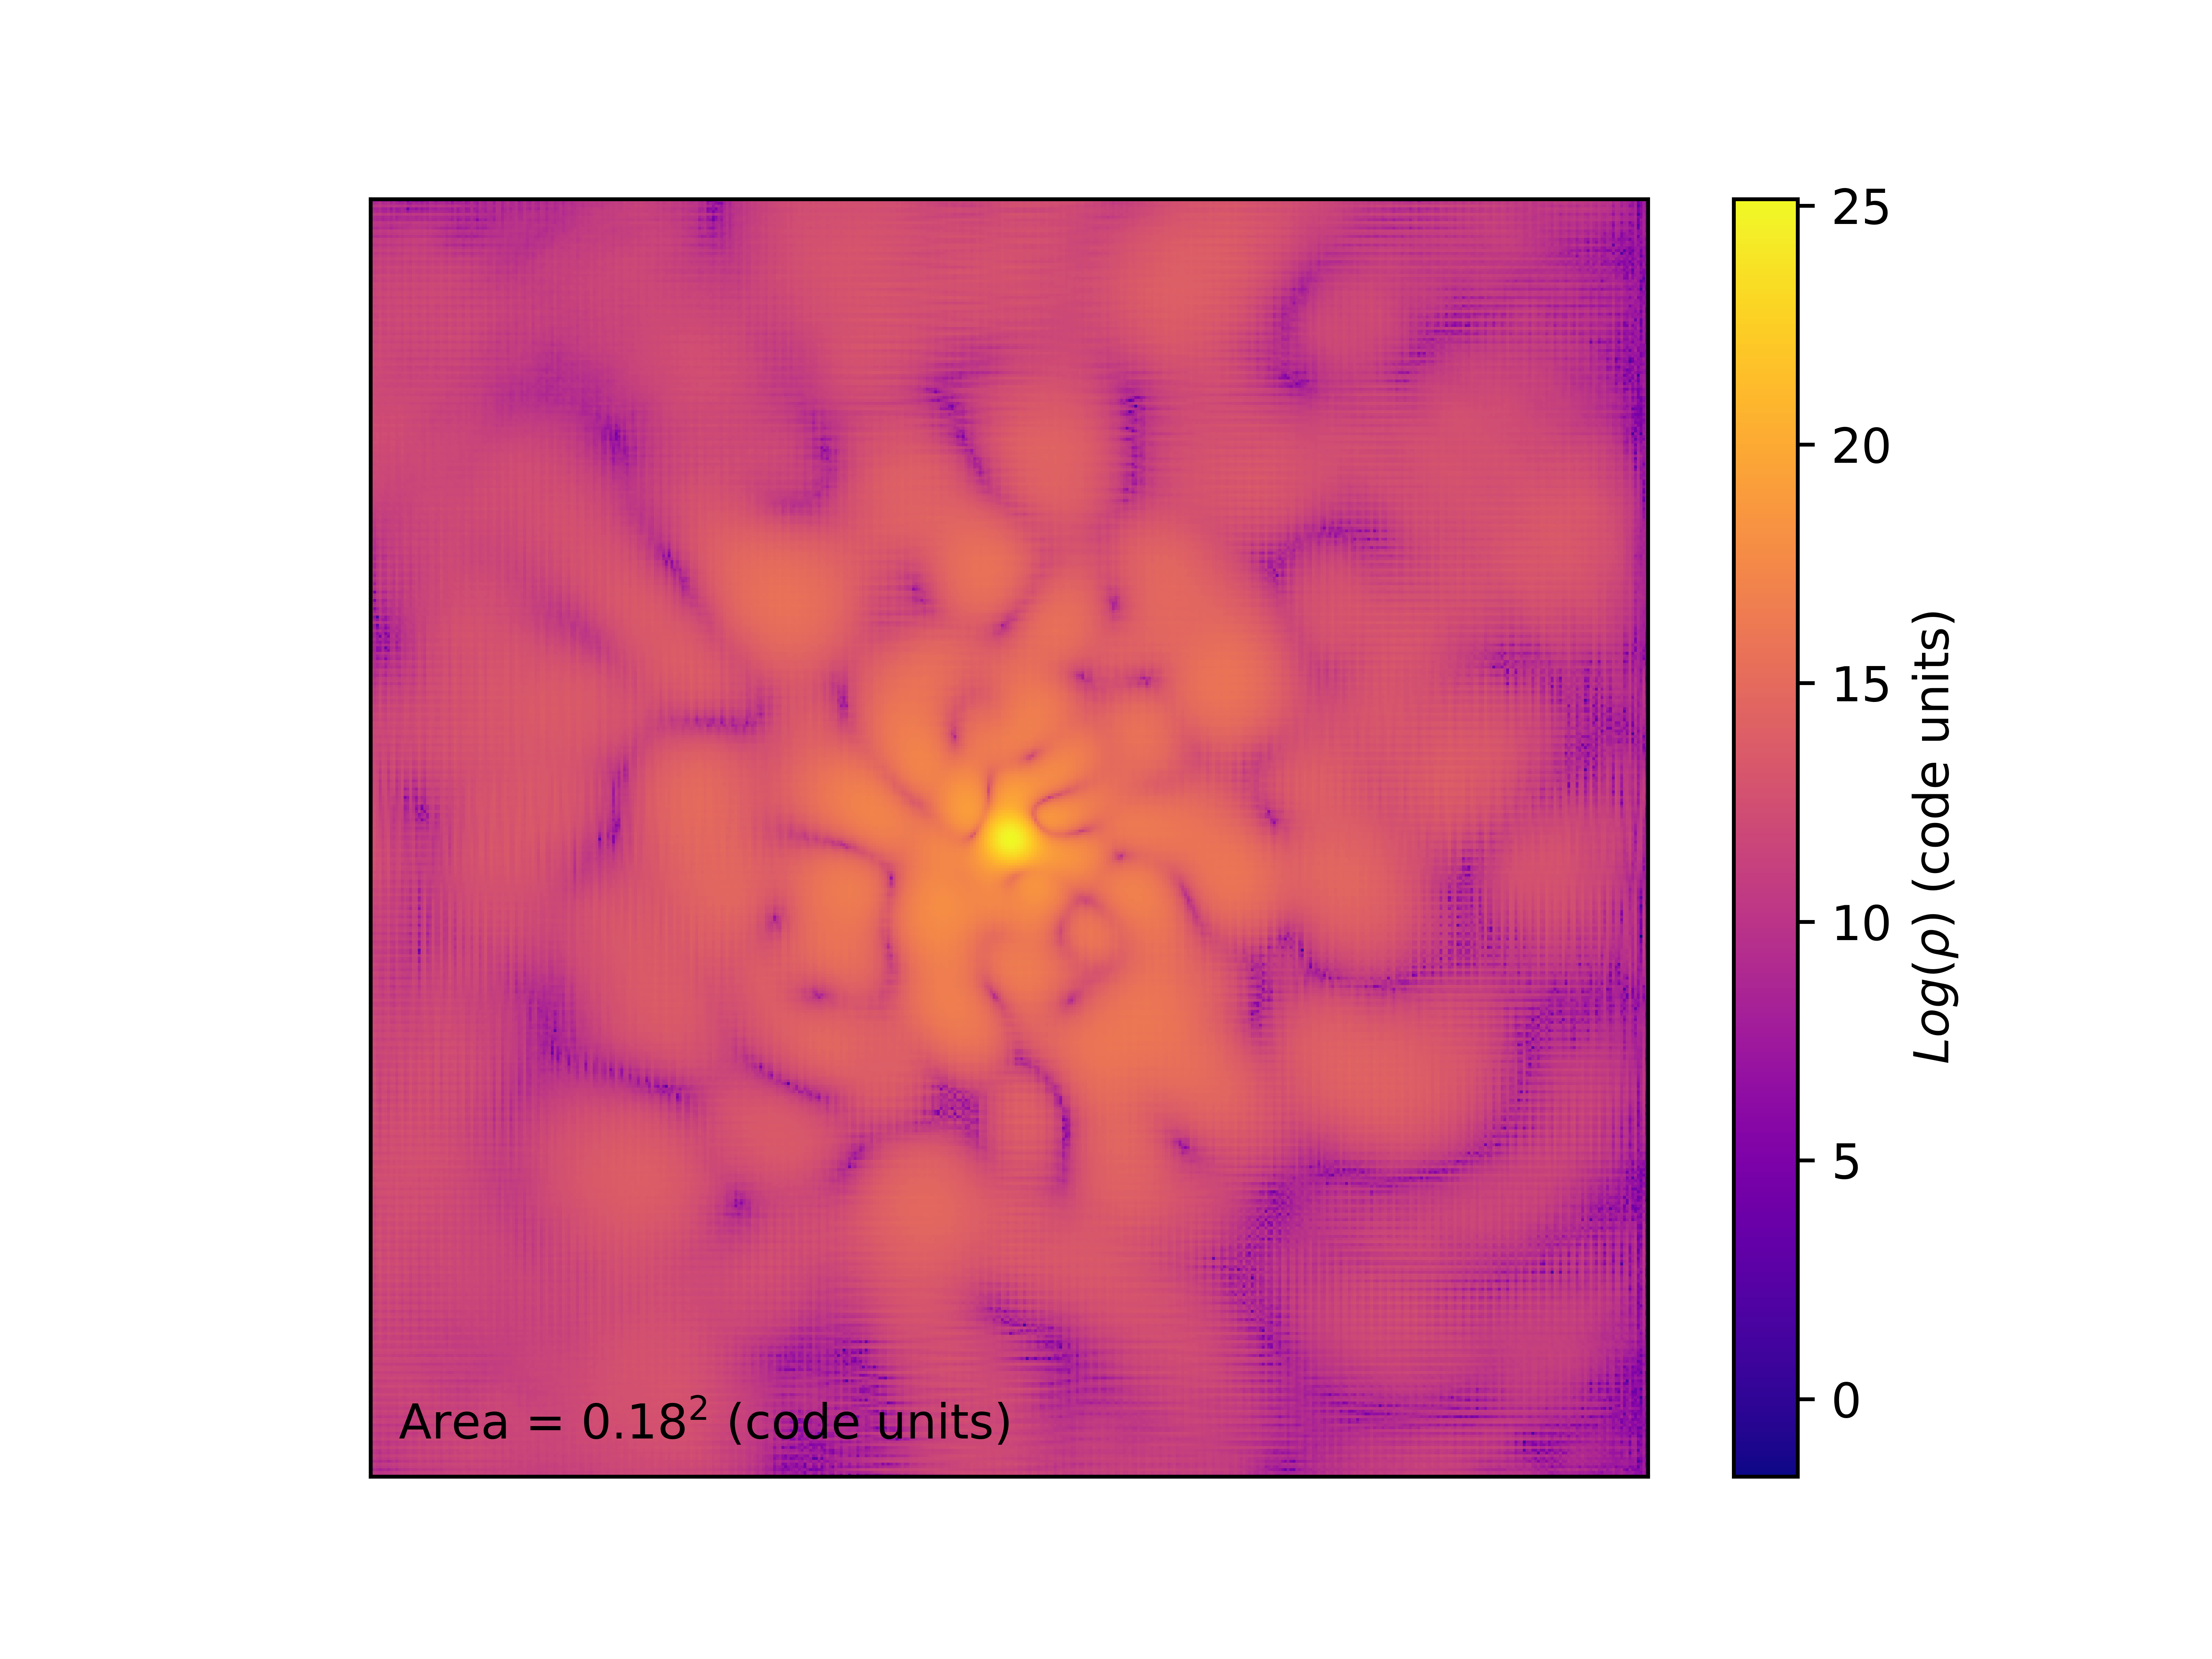
\includegraphics[scale = 0.7, trim={0cm 0cm 0cm 0cm}]{pics/slice.eps}
\caption{Illustration of the scale of the fluctuations present in the turbulent outer halo for the merger product of Figure \ref{fig:pul}. The contour plot represents the (log scaled) local density across a slice through the centre of the final halo. In this plot, distance is not log-scaled, and we see that the spatial size of the fluctuations is of the same order of magnitude as the solitonic core itself.}\label{fig:contour}
\end{figure}

\begin{figure}
% \centering
\begin{tabular}{cc}
{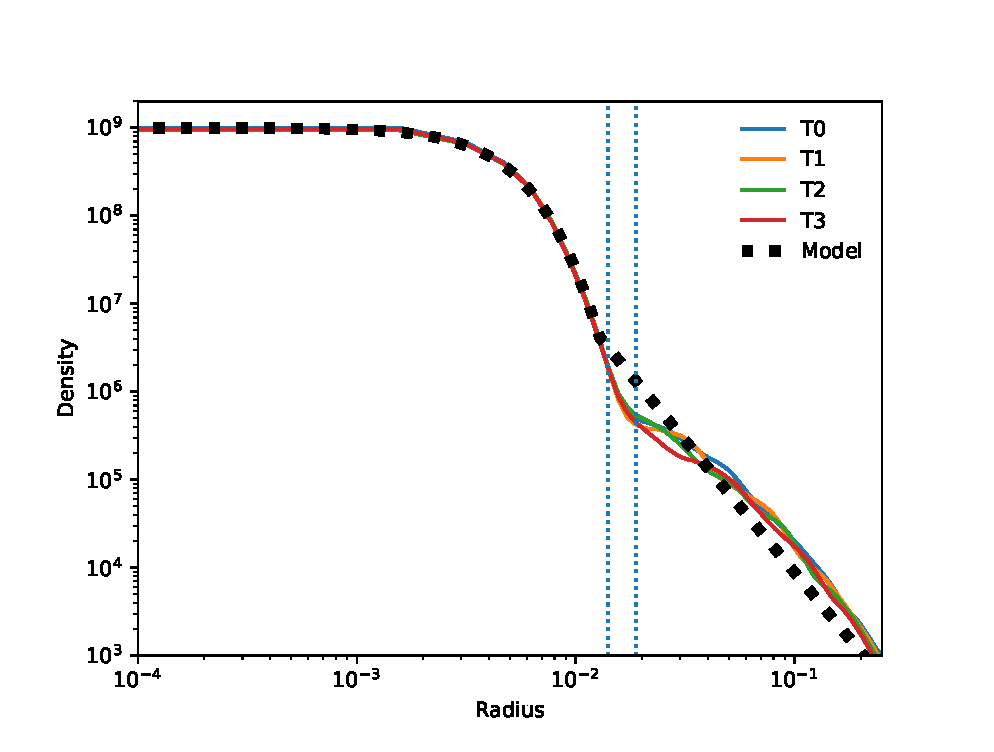
\includegraphics[scale = 0.5, trim={1cm 0cm 1cm 0.35cm}]{pics/combined_small.eps}} &
{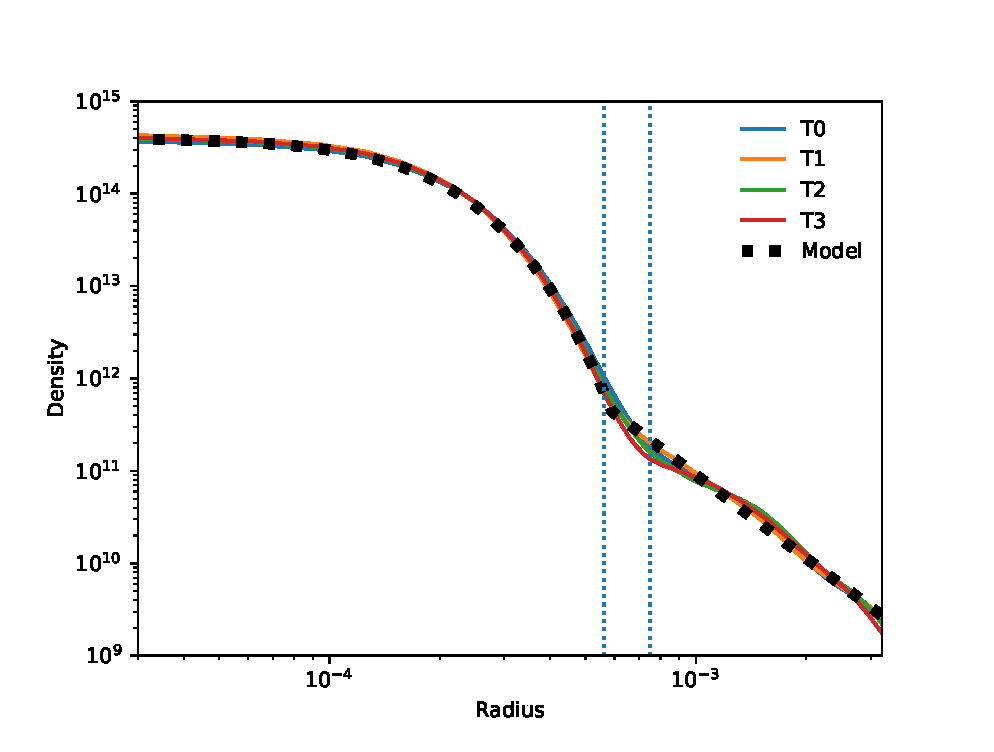
\includegraphics[scale = 0.5, trim={1cm 0cm 1cm 0.35cm}]{pics/combined.eps}}
\end{tabular}
\caption{Left: Merger product of 4 solitons, each with mass 2,000 code units, arranged in a cross configuration. Right: Merger product of 8 solitons of masses $\sim$50,000 code units randomly distributed about the interior of the simulation region. Profiles are plotted for even time intervals from 85\% of total simulation duration, T0 to T4. At these times the halo is relaxed, with changes arising due to turbulence in the outer halo. Profiles are compared to model profiles constructed using the piecewise approach. Good agreement is shown in both cases. Quantities are expressed in dimensionless code units, and vertical dotted lines represent $3r_c$ and $4r_c$.  \re{we should use the same masses in both cases} }\label{fig:validity}
\end{figure}


Halo formation in the ULDM model has been investigated by a number of studies \cite{Schwabe:2016rze, Mocz:2017wlg, Lin:2018whl} which suggest that a generic ULDM halo consists of a solitonic core surrounded by a turbulent outer halo whose density profile falls off like $1/r^3$, as described in the previous Section. Full astrophysical structure formation simulations in ULDM are particularly challenging, given the need to effectively resolve a wide range of scales in an expanding background. However, we can produce ``synthetic'' halos by setting initial conditions in a Schr{\"o}dinger-Poisson  solver corresponding to ${\cal{O}}(10)$ randomly located solitons, allowing them to merge and running the simulation long enough to arrive at a stable ``final'' state. 

We  implemented this approach in {\sc PyUltraLight}  \cite{Edwards:2018ccc}, and the results of one such simulation are shown in Figure \ref{fig:pul}. This profile was obtained through the merger of eight randomly positioned solitons whose masses were selected from within the $\pm 1\sigma$ range of a Gaussian distribution centred at 5000 code units, where $\sigma = 1000$ code units.
The simulation was run at $512^3$ for a duration of 0.05 code units, while the volume of the simulation region, also in code units, was $0.2^3$. The initial positions of the solitons were within the innermost eighth of the total simulation region, ensuring inward gravitational collapse. For ULDM  mass of $10^{-22}\operatorname{eV}$, these choices of simulation parameters correspond to individual progenitor masses of $\sim 1.1*10^{10}\operatorname{M}_{\odot}$, duration $\sim 3.8 \operatorname{Gyr}$, and side length $\sim 7.7 \operatorname{kpc}$. 

The density profile of the resulting merger product is found to be qualitatively similar for larger/smaller progenitor masses, with the size of the solitonic core is subject to the inverse mass-radius scaling relation of the ground-state solution to the Schr{\"o}dinger-Poisson equations. After the solitons collide, some material with large kinetic energy is ejected from the central region. To accommodate this, {\sc PyUltraLight} was modified to include a sponge at the simulation boundary so that this material does not reenter the from the opposite side as a result of the periodic boundary conditions. Hence, mass is not globally conserved. The simulation was run for long enough so that that the mass-loss rate asymptotically approaches zero well before the end of the simulation, giving confidence that the resulting halo represents a relaxed merger product. 

The left panel of Figure \ref{fig:pul} demonstrates the spherically-averaged density profile of the relaxed merger product over time. The inner region is solitonic, transitioning to a $1/r^3$ type profile at a distance of between 3 and 4 times the core radius. We see that while there is some weak time-dependence in the overall profile, it is largely stable. However, the right side panel demonstrates significant local fluctuations in the density of the outer halo along any individual arbitrary direction as function of time. The distance scale of these fluctuations is similar to that of the core itself, as can be seen in Figure \ref{fig:contour}, a feature which is supported by the non-local uncertainty principle invoked in \cite{Schive:2014hza}. The implications of such fluctuations on local tracer velocities have been studied elsewhere \cite{Marsh:2018zyw}, and can provide a useful framework in which to compare the implications of ULDM halo fluctuations with CDM substructure. 

 
While Figure \ref{fig:pul} indicates that simulated ULDM halos do indeed approximate the piecewise generic structure of Equation \ref{eq:piecewise}, we further demonstrate the robustness of this approach by simulating two additional soliton mergers in different mass regimes, under differing initial conditions. The results are shown in Figure \ref{fig:validity}. We see that relaxed halos can be modelled effectively using the piecewise approach across a broad mass range and choice of initial conditions. We note, however, that halo formation from solitonic mergers may differ significantly from halo formation through direct gravitational collapse, and we note also that inclusion of baryonic physics can be expected to lead to significant deviations from DM-only simulations. These limitations should be kept in mind during the below analysis.
 


\section{Comparison of ULDM and CDM halos}\label{sec:ULDM_v_CDM}

\begin{figure}
\begin{tabular}{cc}
{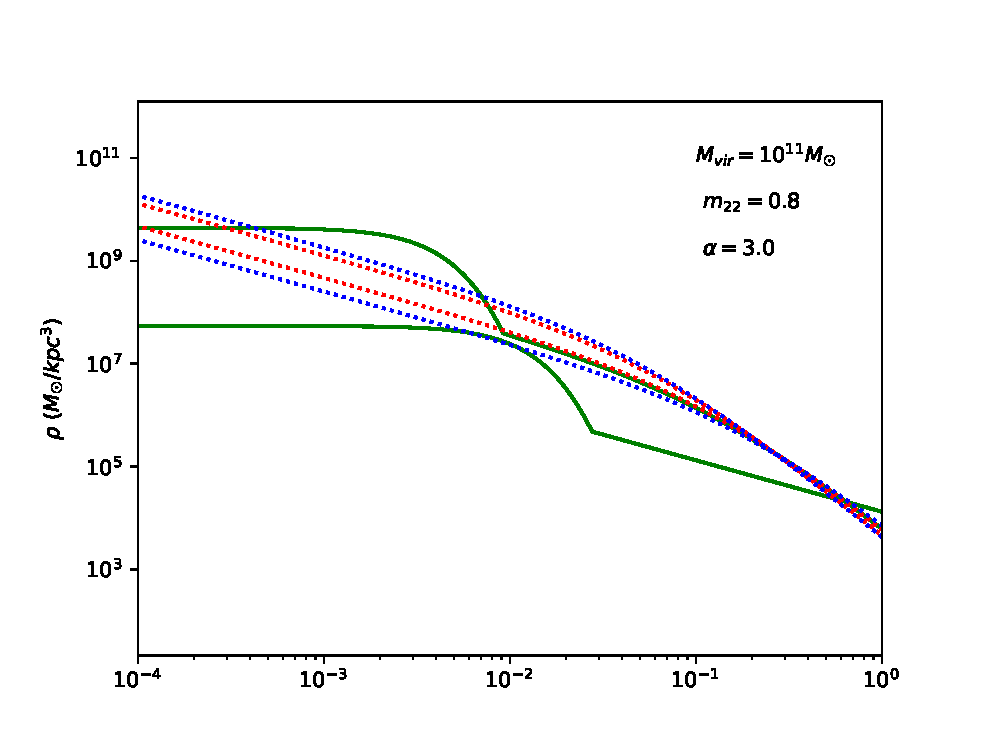
\includegraphics[width = 3.1in, trim={2.1cm 0.5cm 0cm 0.5cm}]{pics/11_8_3.eps}} &
{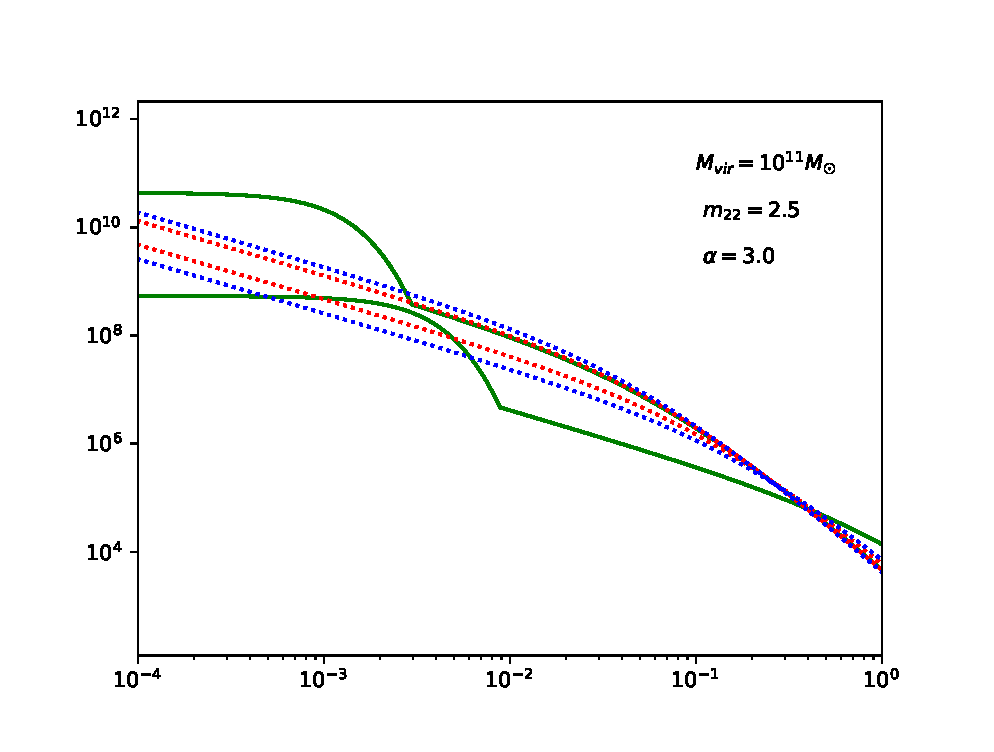
\includegraphics[width = 3.1in, trim={2.1cm 0.5cm 0cm 0.5cm}]{pics/11_25_3.eps}}\\
{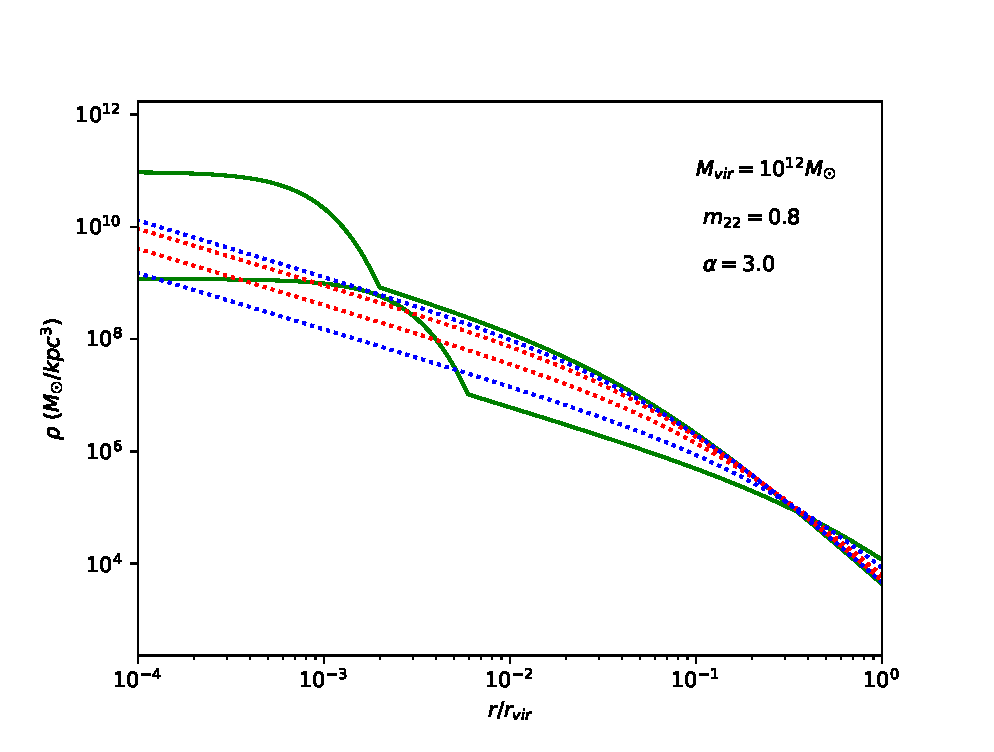
\includegraphics[width = 3.1in, trim={2.1cm 0.5cm 0cm 0.5cm}]{pics/12_8_3.eps}} &
{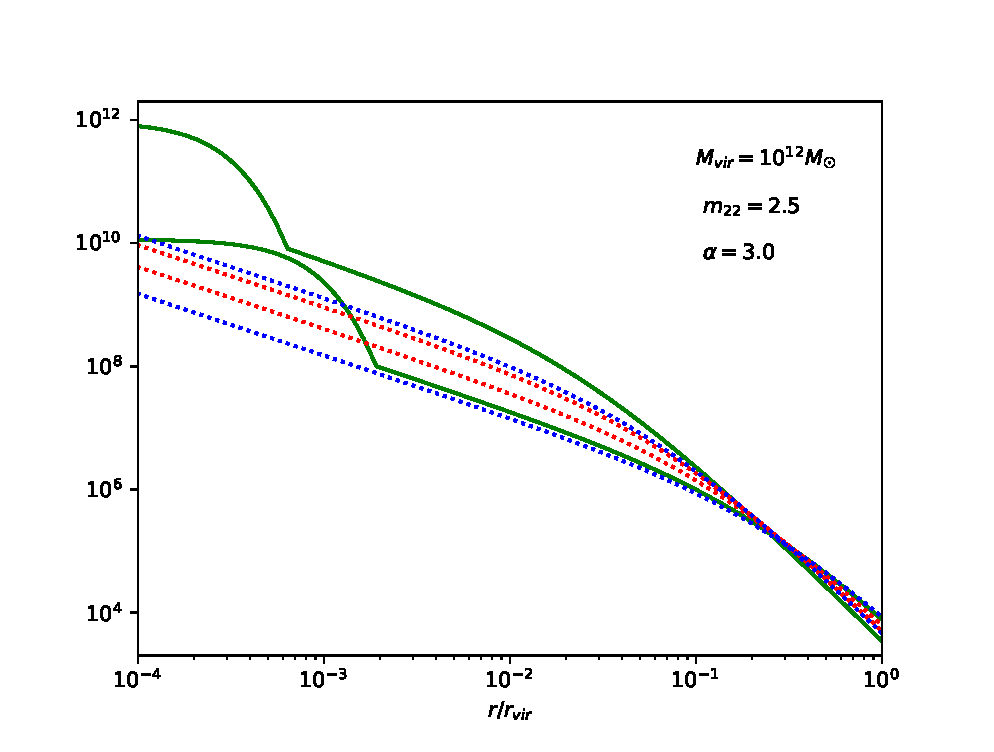
\includegraphics[width = 3.1in, trim={2.1cm 0.5cm 0cm 0.5cm}]{pics/12_25_3.eps}}
\end{tabular}
\caption{Density profiles as a function of radius (normalised to the virial radius) for ULDM and NFW halos of masses $10^{11}\operatorname{M}_{\odot}$ (top) and $10^{12}\operatorname{M}_{\odot}$ (bottom). The left panel represents the results for $m_{22} = 0.8$, while the right panel corresponds to $m_{22}=2.5$. The transition radius is fixed at $r_{\alpha} = 3*r_c$ as its value does not affect the value of the ULDM central density. Green lines represent  ULDM profiles with $\operatorname{M}_c = \operatorname{M}_{cp} \pm 50 \% \operatorname{M}_{cp}$.}\label{fig:profiles}
\end{figure}

 
Using the semi-analytic profiles described above, we now compare the radial profiles of ULDM halos to NFW halos. We focus on masses in the range $10^{11}$ and $10^{12} \operatorname{M}_{\odot}$ since these cases showed an apparent worsening of the core-cusp problem in Ref.~\cite{Robles:2018fur}. Figure \ref{fig:profiles} shows comparisons for representative masses; the green lines represent the ULDM density profiles at the extreme ends of the $\operatorname{M}_c = \operatorname{M}_{cp} \pm 50 \% \operatorname{M}_{cp}$ range, where $\operatorname{M}_{cp}$ is the theoretical predicition for the core mass. Thanks to the scaling relations obeyed by the Schr{\"o}dinger-Poisson soliton solution, this mass range corresponds to a range of $ \gamma_p /4 \geq \gamma \leq 9\gamma_p/4$, where $\gamma_p$ is the theoretical prediction of the square root of the dimensionless central density, yielding a large variation in the central density and widely varying predictions for the overall ULDM profiles. Meanwhile  1-$\sigma$ and 2-$\sigma$ ranges for NFW profiles with different concentrations are show as red and blue dots, respectively \cite{Maccio:2008pcd}. 

Following Ref~\cite{Robles:2018fur}, we plot to a minimum radius of $r/r_{vir} = 10^{-4}$ and for the same choices of $m_{22}$. We note in passing that for any $\operatorname{M}_{vir}$, the NFW halo density at very small radii will inevitably exceed that of the ULDM halo, though the threshold for this transition may be arbitrarily small, and not relevant observationally.  From Figure \ref{fig:profiles} we see that for halo masses of $10^{11}\operatorname{M}_{\odot}$ there is a wide range of $M_c$ for which the ULDM profile is less cuspy than its NFW counterpart.  For a halo mass of $10^{12}\operatorname{M}_{\odot}$ and a ULDM particle mass $m_{22}=0.8$ the ULDM profiles are likewise less peaked than the corresponding NFW profile, but at higher particle mass ($m_{22}=2.5$) the  NFW profiles tend to be less peaked than corresponding ULDM profiles at radial distances in  the range $10^{-4}\leq r/r_{vir} \leq 1$.


\section{Comparison of velocity distributions to SPARC data}\label{sec:velocity}

It is not the dark matter halo density profiles themselves which are imaged directly through astrophysical observations, rather it is the radial velocity distributions of tracer stars. We convert our density profiles to radial velocity distributions \cite{Sofue:2008wt} via 
%
\begin{equation}
    V(r)^2 = \frac{4\pi G}{r}\int_0^r \rho(r')r'^2 dr',
\end{equation}
where 
\begin{equation}
    V^2 = V_{disk}^2 + V_{bulge}^2 + V_{gas}^2 + V_{halo}^2.
\end{equation}
%

We can then compare the resulting velocity distributions to astrophysical data. In this case we will use the SPARC database. This database comprises 175 late-type galaxies, and uses Spitzer photometry at $3.6\operatorname{\mu m}$ to trace the stellar mass distributions.

The disk and bulge velocities in the SPARC database are given for $\Upsilon = 1 \operatorname{M}_{\odot}/\operatorname{L}_{\odot}$ at $3.6\operatorname{\mu m}$. However, the greatest source of uncertainty in mass modelling is the assumption for the stellar mass-to-light ratio, $\Upsilon_\star$ \cite{Lelli:2016zqa}. As in \cite{Robles:2018fur}, we  assume a constant value of $\Upsilon_\star = 0.2 \operatorname{M}_{\odot}/\operatorname{L}_{\odot}$ at $3.6\operatorname{\mu m}$, noting that  this constitutes a non-trivial source of uncertainty in the results. Moreover, there is significant uncertainty in the SPARC data itself, though the error bars are not plotted in the following graphs for ease of viewing. 

\begin{figure}
\begin{tabular}{cc}
{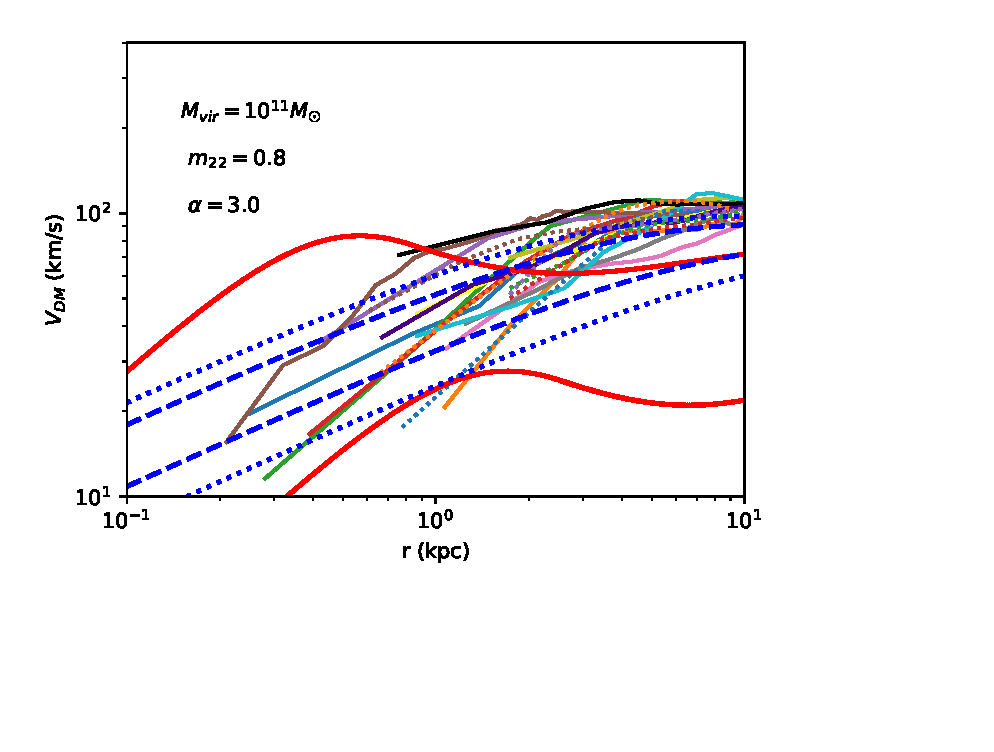
\includegraphics[scale = 0.65, trim={2.5cm 2.5cm 2.1cm 0.5cm}]{pics/v_11_8_3_paper.eps}} &
{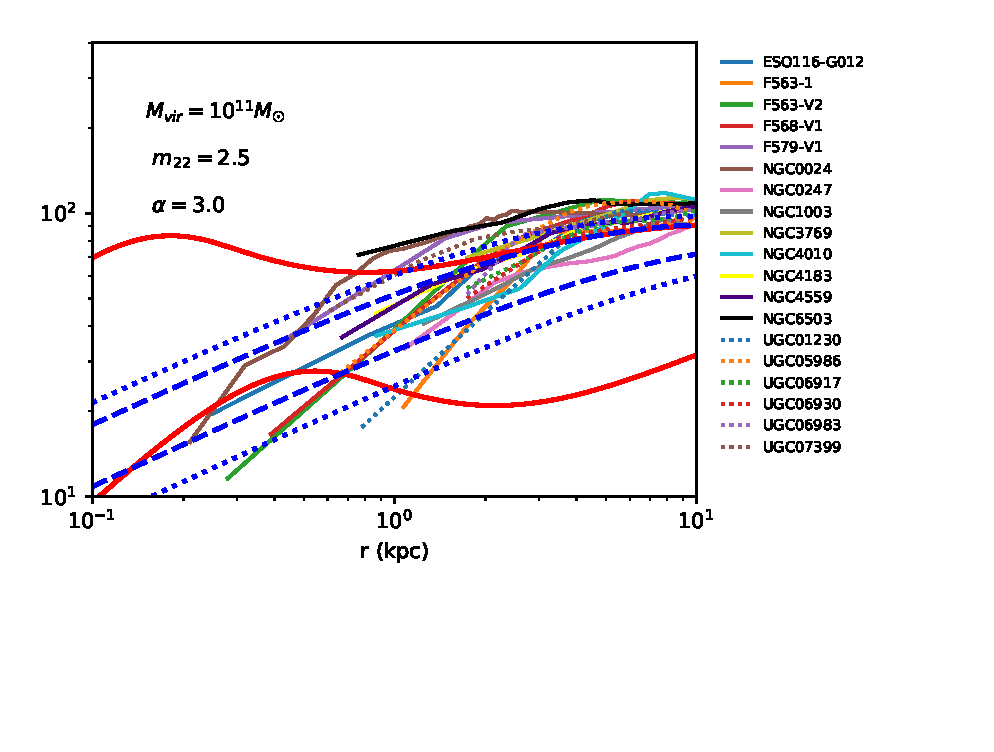
\includegraphics[scale = 0.65, trim={2.1cm 2.5cm 0cm 0.5cm}]{pics/v_11_25_3_paper.eps}}
\end{tabular}
\caption{Theoretical NFW and ULDM velocity profiles for $10^{11}\operatorname{M}_{\odot}$ halos plotted against SPARC data filtered by $V_{max} < 1.2 \operatorname{kms}^{-1}$. Red solid lines represent the extremal ULDM velocity profiles, while  blue dashed and dotted lines represent the 1-$\sigma$ and 2-$\sigma$ NFW bands, respectively. Results are shown for ULDM particle mass $m_{22} = 0.8$ (left) and $m_{22} = 2.5 $ (right). }\label{fig:velocity_11}
\end{figure}


The SPARC database contains photometric data for 175 galaxies, with maximum velocities spanning a range of over $200 \operatorname{kms}^{-1}$. For comparison to the theoretical velocity profiles of the $10^{11}\operatorname{M}_{\odot}$ halos, we have chosen only those candidates with maximum velocity $< 1.2\times 10^2 \operatorname{kms}^{-1}$ and our results are shown in Figures \ref{fig:velocity_11} and \ref{fig:velocity_12}. From Figure \ref{fig:velocity_11}, we see that for $10^{11}\operatorname{M}_{\odot}$  neither  NFW nor  ULDM profiles for appear to show good agreement with the data. While the core-cusp problem is not necessarily exacerbated in the ULDM case, ULDM profiles which roughly fit the data at low radii fall short at larger radii. This problem is worse at larger values of $\alpha$. That said, the proportion of baryonic matter is largest at the centre, so it is in this region that inaccuracies in the assumptions of the stellar mass to light ratio will be most critical.  For this reason it is difficult to determine with certainty which model, if either, is a better fit to the data.

While the SPARC database does not contain any cases for which the velocity is significantly below $10^2\operatorname{kms}^{-1}$ at $10 \operatorname{kpc}$, it would appear that the ULDM profiles for the $10^{11}\operatorname{M}_{\odot}$ halos may provide a better fit to data in a lower velocity regime at this radius.  In Figure \ref{fig:velocity_12}, we show the comparison of the theoretical profiles for the $10^{11}\operatorname{M}_{\odot}$ halos with SPARC data satisfying $1.55 \operatorname{kms}^{-1}\leq V_{max}\leq 2.0 \operatorname{kms}^{-1}$.


\begin{figure}
\begin{tabular}{cc}
{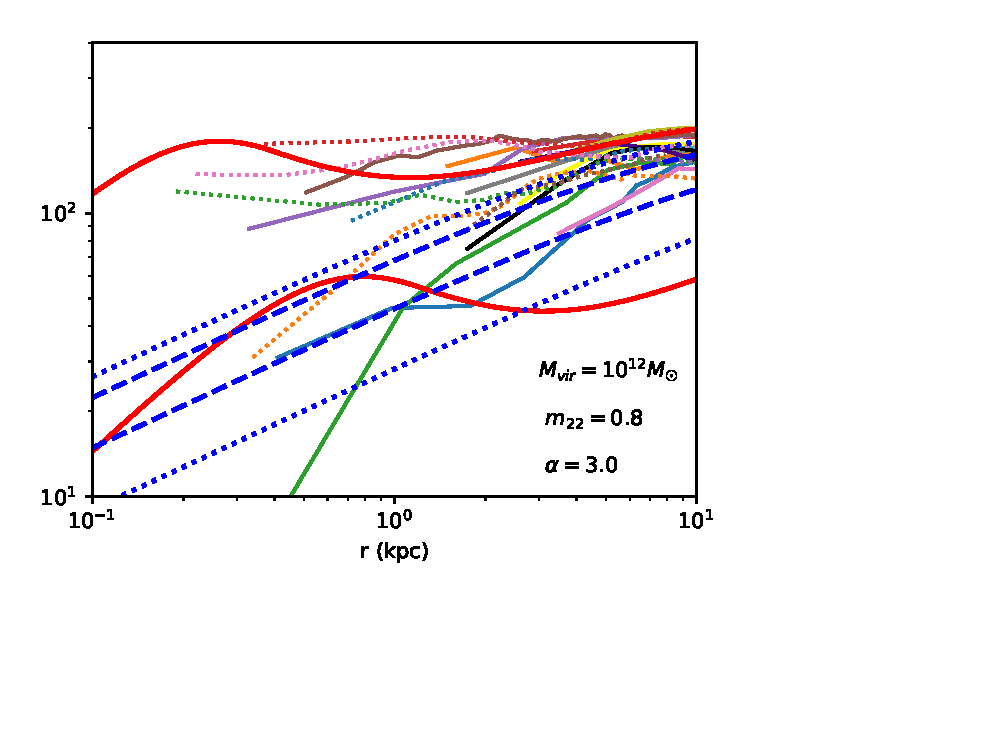
\includegraphics[scale = 0.65, trim={2.5cm 2.5cm 2.1cm 0.5cm}]{pics/v_12_8_3_paper.eps}} &
{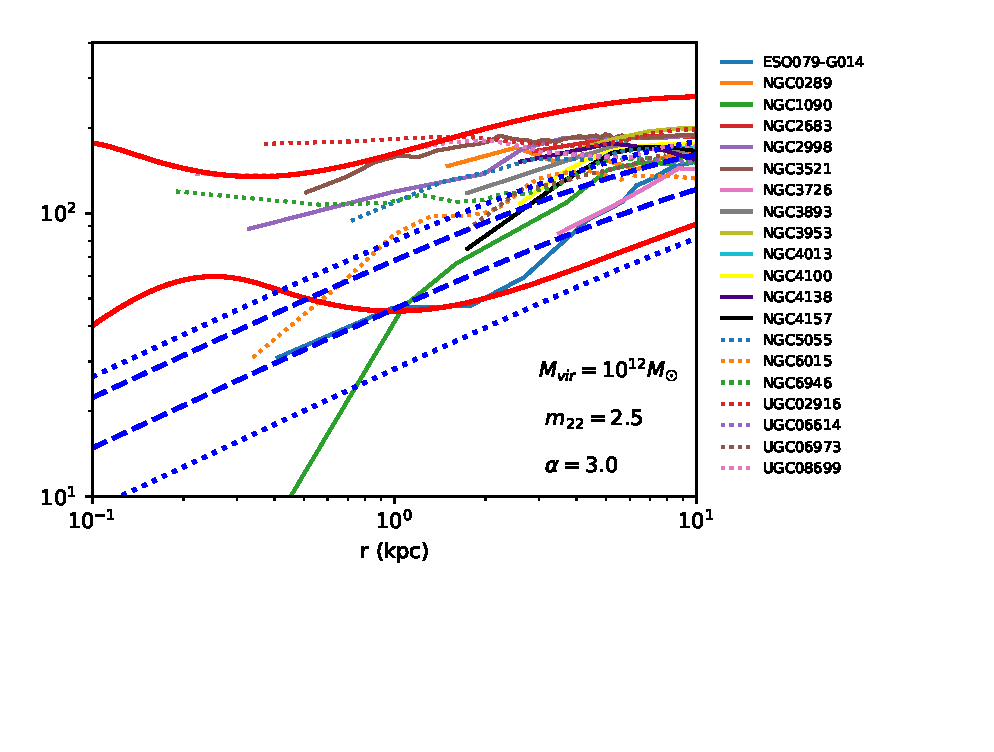
\includegraphics[scale = 0.65, trim={2.1cm 2.5cm 0cm 0.5cm}]{pics/v_12_25_3_paper.eps}}
\end{tabular}
\caption{Theoretical NFW and ULDM velocity profiles for $10^{12}\operatorname{M}_{\odot}$ halos plotted against SPARC data filtered by $1.55 \operatorname{kms}^{-1}\leq V_{max}\leq 2.0 \operatorname{kms}^{-1}$. Red solid lines represent the extremal ULDM velocity profiles, while  blue dashed and dotted lines represent the 1-$\sigma$ and 2-$\sigma$ NFW bands, respectively. Results are shown for ULDM particle mass $m_{22} = 0.8$ (left) and $m_{22} = 2.5 $ (right). \ek{Fits at large radii? Also data doesn't go sufficiently small radius.}}\label{fig:velocity_12}
\end{figure}



As for the $10^{11}\operatorname{M}_{\odot}$ case, neither the ULDM nor the NFW profiles appear to provide a particularly convincing fit to the data. In saying this, it must be recognised that there is significant variation in the trends shown by the data itself, so it would be difficult to find a universally applicable profile. Interestingly, however, there are a number of galaxies in this sample set which have flatter velocity profiles within the plotted range, such as NGC6946, UGC02916, and UGC08699. For these cases, the ULDM profile appears to provide a better fit, however more observational data would be required to confirm this. 

While the ULDM profiles predicted for $10^{11}$ and $10^{12} \operatorname{M}_{\odot}$ halos at $m_{22} = 0.8 - 2.5$ do not provide convincing fits to  the SPARC data, it is interesting to consider models with a slightly lower ULDM particle mass. In particular, if we consider $m_{22} = 0.1$, corresponding to $m = 10^{-23} \operatorname{eV}$, we find a much improved fit to the data. This is shown in Figure \ref{fig:velocity_23}. It should be noted, however, that a ULDM particle mass of this magnitude is in tension with constraints from the Lyman-$\alpha$ forest \cite{Amendola:2005ad}, as well as high-redshift UV luminosity function comparisons \cite{Bozek:2014uqa}. Thus, we ascribe no particular significance to this fit, but note that it serves as an example of how dark matter-only theoretical models may be severely limited in their ability to discriminate between the virtues of competing models.


\begin{figure}
\centering
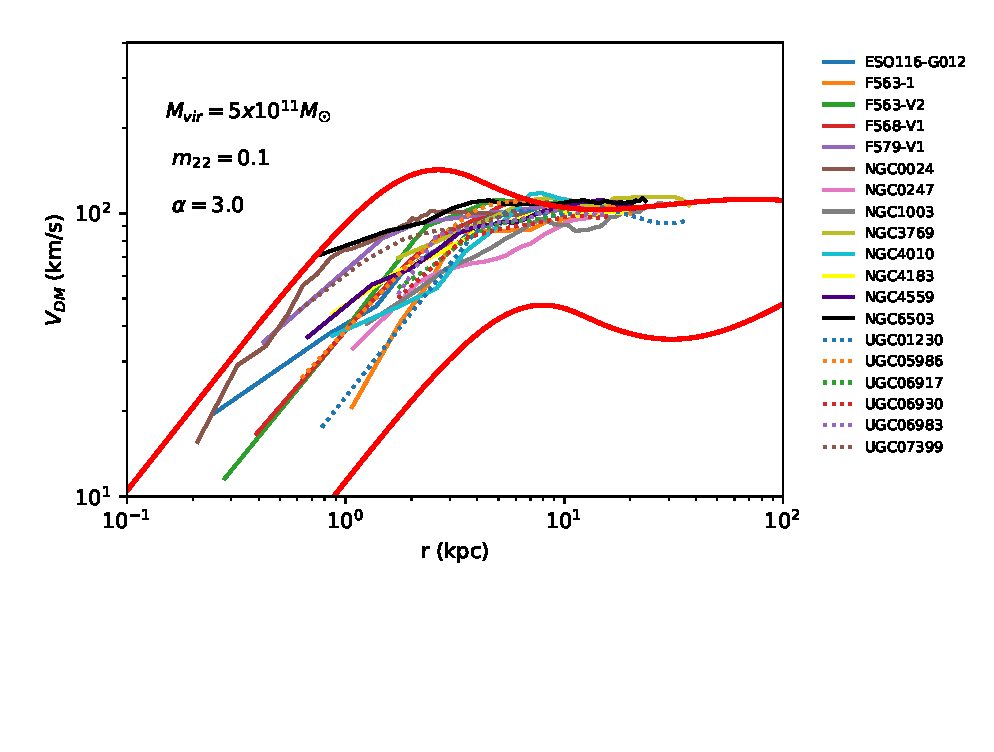
\includegraphics[scale = 0.7, trim={0cm 2.5cm 1cm 0.35cm}]{pics/best_match.eps} 
\caption{Range of theoretical ULDM profiles for a halo of mass $5\times 10^{11}\operatorname{M}_{\odot}$ and virial radius 200kpc with $m_{22} = 0.1$. Also plotted are the SPARC data satisfying $V_{max}\leq 1.2 \operatorname{kms}^{-1}$. \ek{slightly higher mass?}}\label{fig:velocity_23}
\end{figure}


\section{Conclusions}\label{sec:conclusion}

While the ULDM model has gained popularity as a means by which to resolve the contentious core-cusp problem of CDM, there exist cases in which theoretical ULDM profiles have higher densities than their NFW counterparts at observationally relevant radii in the interior of massive dwarf galaxies. However, given the apparent spread in the predicted ULDM core-halo mass relation \cite{Schive:2014hza}, there exists a sizeable range of plausible central densities for a halo of any given mass. Analysis of oscillations of the cores of ULDM halos on timescales much smaller than the relaxation time have also demonstrated significant fluctuations in central density \cite{Veltmaat:2018dfz}. These observations suggest that the theoretical core-halo mass relation of ULDM should not be interpreted too literally for any individual halo, but be viewed as a statistical feature of halo formation. In some circumstances, choosing a core mass at the lower end of the plausible range can mitigate the apparent core-cusp discrepancy. 

With spread around the predicted core-halo relation in mind, comparison of theoretical ULDM and NFW profiles to photometric data from the SPARC database yields inconclusive results, as neither ULDM nor NFW profiles provide a particularly good fit to the data in the ranges $10^{11}\operatorname{M}_{\odot}\leq \operatorname{M}_{vir} \leq 10^{12}\operatorname{M}_{\odot}$ and $0.8 \leq m_{22} \leq 2.5$. Interestingly, however, a better fit to the lower velocity SPARC data is obtained from a ULDM profile where $m_{22} = 0.1$ and $\operatorname{M}_{vir} = 5\times 10^{11}\operatorname{M}_{\odot}$. It must be noted, however, that such a small ULDM particle mass appears to be in tension with current constraints \cite{Amendola:2005ad, Bozek:2014uqa, Armengaud:2017nkf, Ni:2019qfa, Nebrin:2018vqt}. Tightening these constraints on the plausible ULDM particle mass, as well as constraints on the fraction of dark matter accountable for by ULDM is the subject of ongoing research, and will inform future investigations of this type \cite{Castellano:2019hdd, Lidz:2018fqo, Davoudiasl:2019nlo}.


It is clear that more data, both from simulations and astrophysical observations, is required to fully explore the applicability of the ULDM model of dark matter. The parameter space used to describe `typical' ULDM halos appears to be larger than simple semi-analytical models would suggest, and must ultimately include elements of baryonic feedback. Furthermore, a larger volume of photometric data with improved uncertainties and covering a greater halo mass range would be of tremendous benefit in determining the suitability of ULDM. Indeed, it is reasonable to expect a vast amount of new data becoming available in the near future, as a number of extensive surveys are undertaken \cite{Simon:2019kmm}. In addition, cosmological structure formation simulations for ULDM models continue to be an active area of research \cite{Lin:2018whl, Clough:2018exo, Mocz:2015sda}, and we can expect an improvement on the statistics surrounding ULDM halo formation in future. Thus, while this preliminary work is somewhat inconclusive, it motivates further analyses of this kind in future as available datasets advance. 




\acknowledgments

We acknowledge invaluable discussions with Jens Niemeyer, Shaun Hotchkiss, and Mateja Gosenca in completing this work. We also acknowledge support from the Marsden Fund of the Royal Society of New Zealand. This research was supported by use of the Nectar Research Cloud, a collaborative Australian research platform supported by the National Collaborative Research Infrastructure Strategy (NCRIS).





\bibliographystyle{JHEP-mod}
\bibliography{refs} 


\end{document}
